\documentclass{beamer}

\mode<presentation>{\usetheme{Warsaw}}
\title{Deep Learning Enhanced Mobile-Phone Microscopy 阅读报告}

\author{报告人:宋明辉}

%\logo{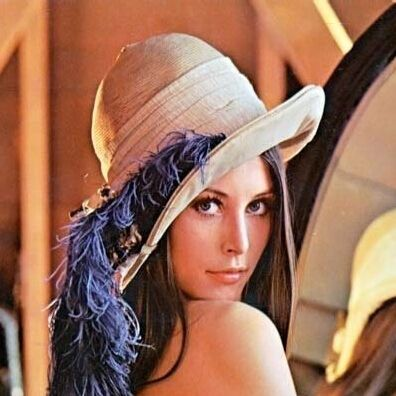
\includegraphics{lena.jpg}}

\usepackage{xeCJK}
\setmainfont{Times New Roman}
\setCJKmainfont[AutoFakeBold, ItalicFont={SimSun}]{KaiTi}
\setCJKsansfont{SimHei}
\setCJKmonofont{SimSun}
\usefonttheme{serif}

\usepackage{algorithm}
\usepackage{algorithmicx}
\usepackage{algpseudocode}

\usepackage{graphicx}
\usepackage{subfigure}
\usepackage{xcolor}

\usepackage{amsmath}
\usepackage{booktabs}
\usepackage{multirow}

\renewcommand{\figurename}{Fig.}
\renewcommand{\tablename}{Table.}
\setbeamertemplate{caption}[numbered]

\begin{document}
% \captionsetup[Figure:]{labelfont={bf}, labelformat={default}, labelsep=period, name={Fig.}}

\frame[plain]{
\titlepage
}

\begin{frame}{报告内容}
\tableofcontents[
sectionstyle=show/show,
subsectionstyle=hide/hide/hide
]
\end{frame}

\AtBeginSection{
\begin{frame}
\tableofcontents[
currentsection,
]
\end{frame}
}

\section{目的}

\begin{frame}
\frametitle{目的}

\begin{columns}
\column{0.5\textwidth}
\begin{figure}
\centering
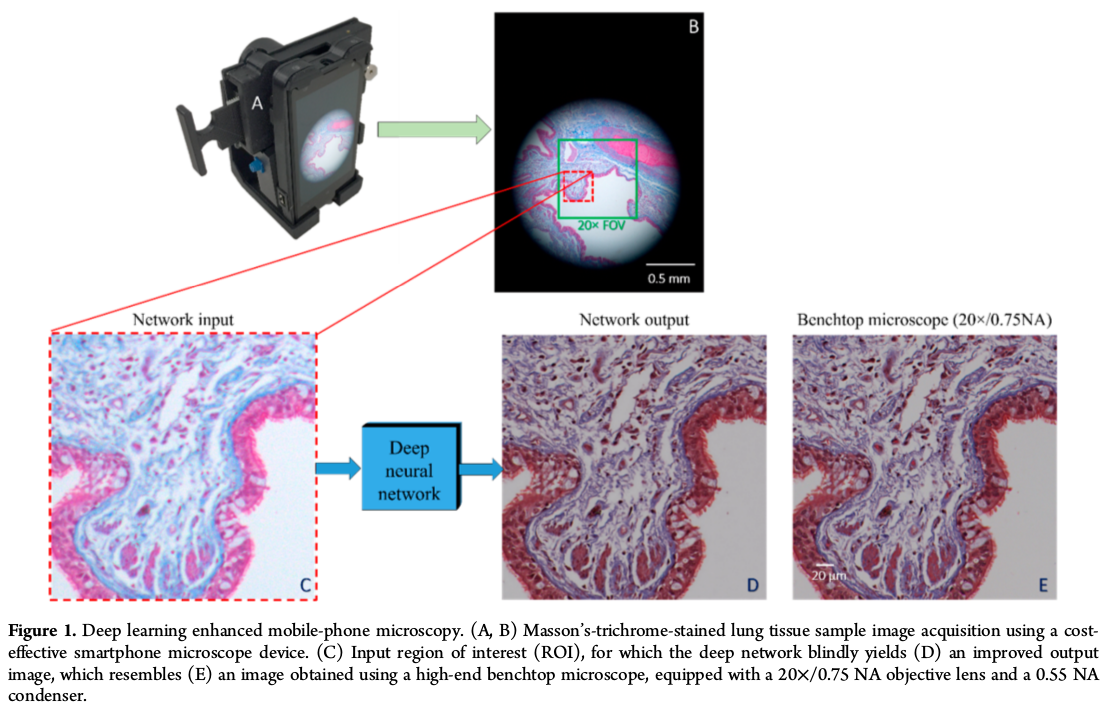
\includegraphics[width=0.9\textwidth]{Diagram1.png}
%\insertcaptionname{Fig. 目的}
\caption{示意图} 
\end{figure}
\textbf{注意:}
\textbf{输入图像}为通过手机相机得到的图像,\textbf{输出图像}特指经神经网络处理得到的图像,\textbf{目标图像}为通过显微镜得到的图像。

%\pause
\column{0.5\textwidth}
%\pause
%\textbf{目的:}
目的:
\begin{itemize}
\item 借助深度学习将低成本手机相机的图像增强到与昂贵显微镜的图像相似的分辨率
\item 消除输入图像中的噪声、色彩失真等
\item 作为一种标准化手段,便于其它医学应用
\end{itemize}

总而言之,利用低成本、便捷的成像设备,如手机等,代替昂贵、繁杂的专业显微镜。


\end{columns}

\end{frame}

\section{成像设备对比}
\begin{frame}
\frametitle{成像设备对比}
\begin{table}[!t]
\centering
\begin{tabular}{ccc}
\toprule
参数 & 手机相机\footnote{Nokia Lumia 1020}    &    专业显微镜\footnote{Olympus IX83} \\
\midrule
数值孔径(NA)  &  较低    &  0.75 \\
Pixel Size($\mu m$)   &  1.12  & 7.4 \\
FOV\footnote{Field of View}($mm^2$) & $\sim$1  & 0.57 \\
曝光时间(s)  & 1/49 $\sim$ 1/13   & 未知 \\
\bottomrule
\end{tabular}
\end{table}

因此,相比于显微镜,手机图像具有以下缺点:
\begin{itemize}
\item 分辨率较低
\item 敏感性较低,易引入噪声、色彩失真
\end{itemize}

\end{frame}

\section{提出的算法}

\subsection{数据预处理}

\begin{frame}
\frametitle{预处理的内容}
根据实验目的、上述对成像设备的成像特点分析,预处理需要完成以下内容:
\begin{itemize}
\item FOV匹配 \\
即需要保证观察的内容是一致的,否则,计算得到的增强算法就是错误的。

通过 \textbf{计算单应矩阵} 完成。
\item 图像配准\\
需要保证在更细小结构上的对应。神经网络作用于配准后的图像,这样可以保证学习\textbf{输入图像}与\textbf{目标图像}之间的失真关系。

这部分基于 \textbf{局部矫正} 完成。
\item 上采样,这部分由神经网络的最后一层卷积层完成。便于网络的训练、以及保证网络结构的精简。
\end{itemize}

\end{frame}

\begin{frame}
\frametitle{计算单应矩阵}

根据单应矩阵的定义,主要消除因旋转、形变、平移等因素引起的不匹配,表现形式为$3\times3$的矩阵,对输入图像进行线性变换。这一步开始之前,需要将输入图像转换成TIFF格式或JPEG格式。

主要计算流程(经典实现方式):
\begin{itemize}
\item 计算SIFT特征({\color{red} 目前来说,应该最优的特征检测算法,或许可以换成计算效率更高的算法})
\item 基于RANSAC算法计算特征的之间的匹配关系
\item 基于匹配的特征点计算单应矩阵
\end{itemize}
这一步完成后,得到全局匹配(Globally Matched)的图像对。
\end{frame}

\begin{frame}
\frametitle{局部配准}
基于 Pyramid Elastic Registration Algorithm 完成
\begin{columns}
\column{0.75\textwidth}
\begin{figure}
%\raggedright
\centering
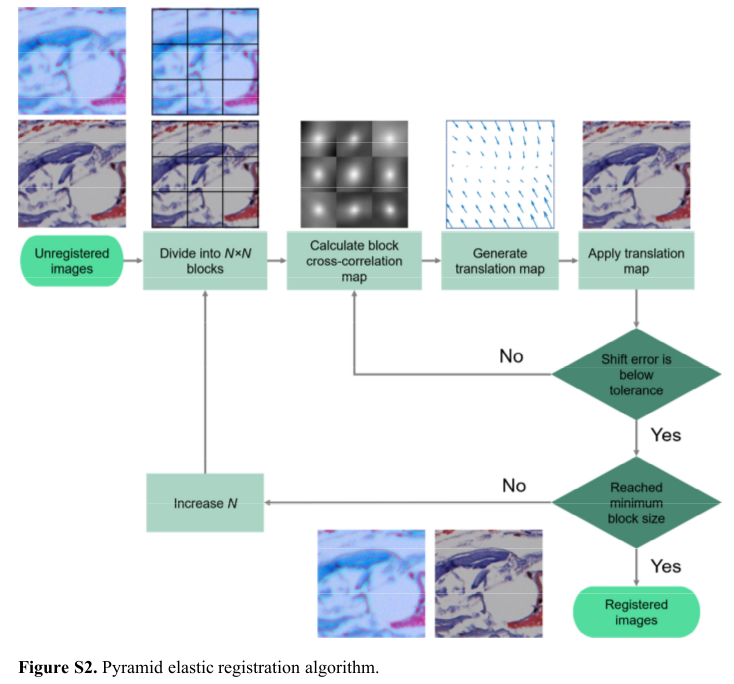
\includegraphics[width=0.8\textwidth]{Pyramid.png}
\end{figure}

\column{0.4\textwidth}
主要步骤:
\begin{itemize}
\item 将输入图像、目标图像迭代地分割成N * N大小的Block
\item 计算对应Block的Cross-Correlation(互相关)
\item 计算转换图(Translation Map)
\item 根据转换图对Block进行处理(线性变换)
\end{itemize}

\end{columns}
\end{frame}

\subsection{神经网络结构}

\begin{frame}
\tableofcontents[
sectionstyle=show/show,
subsectionstyle=show/share/hide,
currentsubsection,
]
\end{frame}

\begin{frame}
\frametitle{概览}
\begin{figure}
\centering
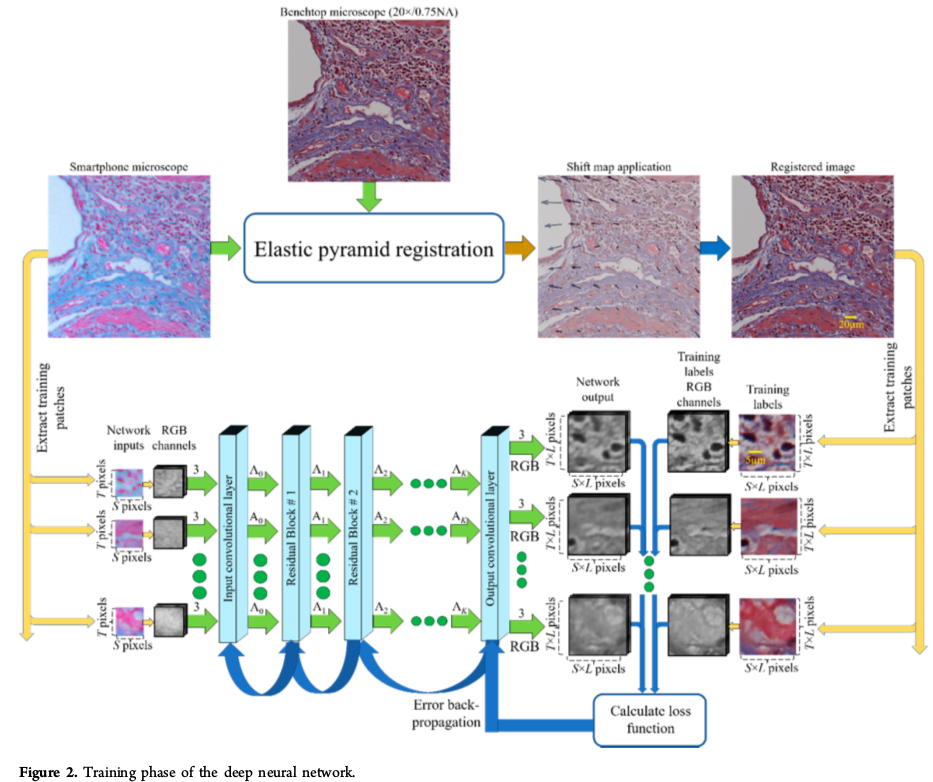
\includegraphics[width=0.6\textwidth]{Training.png}
\end{figure}
有监督学习:输入为手机成像结果,Label为显微镜成像结果

基本的卷积块: 残差块(Residual Blocks)
\end{frame}

\begin{frame}
\frametitle{网络结构1}
Residual Block:
\begin{figure}
%\raggedright
\centering
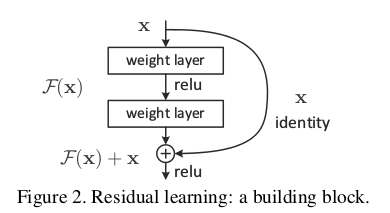
\includegraphics[width=0.5\textwidth]{Residual.png}
\end{figure}

数学表达式:
\begin{displaymath}
\centering
X_{k+1}=X_{k} + ReLU(Conv_{k_2}(ReLU(Conv_{k_1}(X_k)))))
\end{displaymath}

卷积核大小:$3 \times 3$
\end{frame}

\begin{frame}
\frametitle{网络结构2}
各个Residual Block的Feature map数量:
\begin{displaymath}
A_k = A_{K_1} + floor((\alpha \times k)/K + 0.5)
\end{displaymath}
其中,$K=5$, $k=[1:5]$, $\alpha=10$, $A_0 = 32$.
\vspace{1cm}
\par Upsampling:

最后一层卷积层输出3个通道,分别对应R、G、B三个通道;同时完成升采样的过程:不清楚是通过Deconvolution还是其它的方式实现。

\end{frame}


\begin{frame}
\frametitle{损失函数}
损失函数为MSE(均方误差:Mean-Squared Error) 与 一个正则项的和:
%\begin{displaymath}
\begin{multline}
l(\theta) = \frac{1}{3 * S * T * L^2} \left[
\sum_{c=1}^{3}\sum_{s=1}^{S * L}\sum_{t=1}^{T * L} \parallel Y_{c, s, t}^{\theta} - Y_{c, s, t}^{Label} \parallel^2 + \right. \\
\left. \lambda \sum_{c=1}^{3}\sum_{s=1}^{S * L}\sum_{t=1}^{T * L}| \nabla Y^{\theta} |_{c, s, t}^2 \right]
\end{multline}
%\end{displaymath}
其中正则项为\textbf{输出图像}梯度幅度的平方,$\lambda=0.001$.

\vspace{6pt}
训练:Adam

\end{frame}



\subsection{评价指标以及实验结果}
\begin{frame}
\frametitle{评价指标、实验结果}
\begin{table}
\begin{tabular}{c|c|c}
\toprule
评价指标  &  Color Distance (CIE空间)   &   SSIM\footnote{Structural Similarity} \\
\bottomrule
\end{tabular}
\end{table}

\begin{figure}
\centering
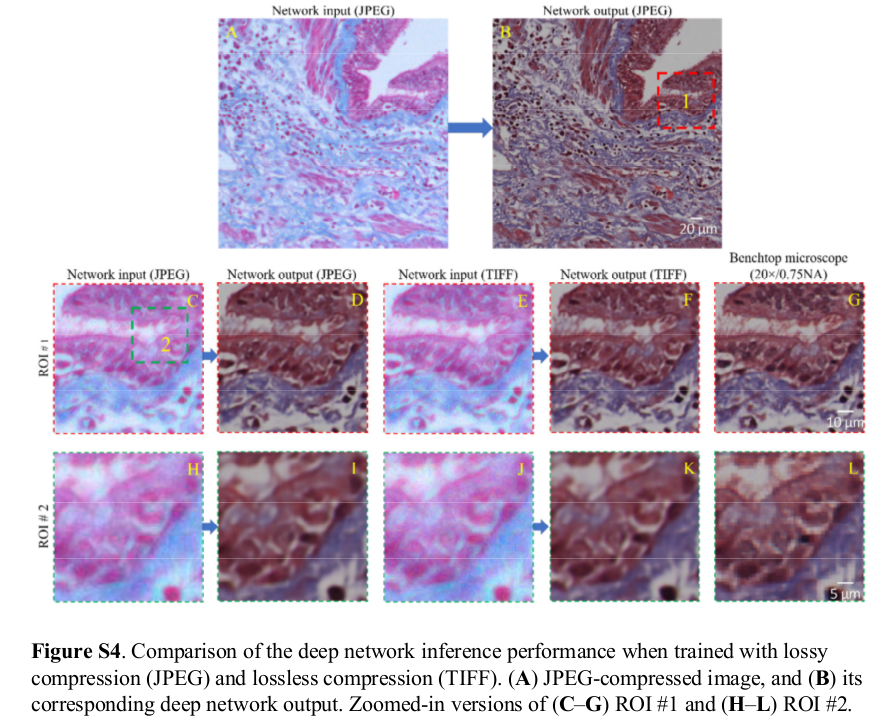
\includegraphics[width=0.6\textwidth]{Results.png}
\end{figure}

\end{frame}


\section{分析与总结}

\begin{frame}
\frametitle{优势与不足}
\begin{itemize}
\item 优势
\begin{itemize}
\item 可以方便的以迁移学习的方式,部署到其它基于手机的成像系统中
\item 输入图像可以为有损压缩后的图像(如JPEG),方便存储以及传输等
\item 结果表明,以深度学习为工具可以实现预定目标
\end{itemize}
\item 不足
\begin{itemize}
\item 为什么选择以残差块(ResNet)形式的神经网络结构(透明性?)
\item 目标函数(其它的类型是否有效)
\item 为了保证网络的精简,一些工作由预处理完成,或许可以设计统一的端到端学习结构
\end{itemize}
\end{itemize}

\end{frame}

\begin{frame}[plain]

{
\Large
\bfseries
\begin{center}
\color{orange}请各位\color{green}老师、同学\color{blue}批评指正!
\end{center}
}

\end{frame}

\end{document}

